
\documentclass[tikz]{standalone}

\usetikzlibrary{arrows,shapes,automata,petri,positioning}
\usepackage{xcolor}
\definecolor{darkblue}{rgb}{0.2,0.2,0.6}
\definecolor{darkred}{rgb}{0.6,0.1,0.1}
\definecolor{darkgreen}{rgb}{0.2,0.6,0.2}

\definecolor{acsiorange}{RGB}{180,88,26}
\definecolor{acsired}{RGB}{150,0,0}
\definecolor{acsigreen}{RGB}{128,198,54}
\definecolor{acsiblue}{RGB}{43,80,150}

%%%%%%%%%%%%%%%%%%%%%%%%%%%%%%%%%%%%%%%%
\definecolor{swimmyred}{RGB}{206,19,55}
\definecolor{marcofucsia1}{RGB}{203,41,123}
\definecolor{marcofucsia1}{RGB}{203,41,123}
\definecolor{marcofucsia2}{RGB}{153,25,94}
\definecolor{marcofucsia3}{RGB}{102,29,70}
\definecolor{marcoblue1}{RGB}{17,183,225}
\definecolor{marcoblue2}{RGB}{16,163,201}
\definecolor{marcoblue3}{RGB}{5,132,165}
\definecolor{marcoblue4}{RGB}{4,105,131}
\definecolor{marcoblue5}{RGB}{0,77,128}
\definecolor{marcoorange}{RGB}{255,147,0}
\definecolor{marcogreen1}{RGB}{82,174,139}
\definecolor{marcogreen2}{RGB}{56,122,101}


\newcommand{\tcolor}{\color{darkgreen}}
\newcommand{\wcolor}{\color{marcofucsia1}}
\newcommand{\pcolor}{\color{violet}}

%%%%%%%%%%%%%%%%%%% PETRI %%%%%%%%%%%%%%%%%%%%%%%%
\usetikzlibrary{arrows,shapes,automata,petri,positioning,calc}

\tikzset{
	place/.style={
		circle,
		very thick,
		draw=acsiblue!90,
		fill=acsiblue!10,
		minimum size=6mm,
	},
	transitionH/.style={
		rectangle,
		thick,
		fill=black,
		minimum width=6mm,
		inner ysep=2pt
	},
	transitionV/.style={
		rectangle,
		thick,
		fill=black,
		minimum height=6mm,
		inner xsep=2pt
	},
    tau/.style={
      fill=gray,
    },
    arc/.style={
        -angle 90,
        thick,
    },
	state/.style={
		rectangle,
        rounded corners=5pt,
        draw,
		very thick,
		fill=orange!10,
		minimum height=5mm,
		minimum width=10mm,
	},
    link/.style={
        -stealth,
        thick,
    },
	config/.style={
		circle,
        rounded corners=5pt,
        draw,
		very thick,
        fill=black,
		minimum height=2mm,
		minimum width=2mm,
        font=\tiny\color{white}
	},
    hconfig/.style={
		circle,
        rounded corners=5pt,
     	minimum height=2mm,
		minimum width=2mm,
        font=\tiny\color{white}
	},
}



\tikzstyle{joint}=[
 	circle,
	minimum size=1mm,
    draw,
    very thick,
]

\tikzstyle{cjoint}=[
    joint,
    fill=marcoorange!80,
]

\tikzstyle{pjoint}=[
    joint,
    fill=marcoorange!30,
]

\tikzstyle{cstep}=[
    rectangle,
    rounded corners=5pt,
    minimum height=3.5em,
    minimum width=5em,
    very thick,
    draw,
    fill=marcoblue1!40,
    font=\footnotesize
]

\tikzstyle{astep}=[
    rectangle,
    minimum height=4.2em,
    minimum width=5em,
    thick,
    draw,
    fill=marcoblue2!20,
    inner sep=5,
]

\tikzset{database/.style={cylinder,aspect=0.5,draw,rotate=90,path picture={
			\draw (path picture bounding box.160) to[out=180,in=180] (path picture bounding
			box.20);
			\draw (path picture bounding box.200) to[out=180,in=180] (path picture bounding
			box.340);
}}}



\begin{document}
	
	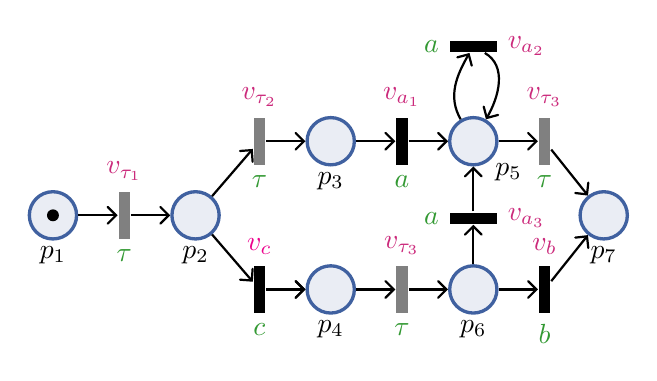
\begin{tikzpicture}[node distance=0.4cm and 0.5cm,>=stealth',bend angle=45,auto]
	\node [place,tokens=1] (i) {};
    \node [below=-0.5mm of i] {$p_1$};
	\node [
      transitionV,
      tau,
      right= of i,
      label=below:$\tcolor\tau$,
      label=above:$\wcolor v_{\tau_1}$,
    ] (t1) {};
	\node [
      place,
      right=of t1
    ] (p2){};
    \node [
      below=-0.5mm of p2
    ] {$p_2$};
	\node  (b1) [right=of p2] {};
	\node  (b2) [right=of b1] {};
	\node [
      transitionV,
      tau,
      above right=of p2,
      label=below:$\tcolor \tau$,
      label=above:$\wcolor v_{\tau_2}$,
    ] (te1) {};
	\node [
      place, 
      right=of te1
    ] (p3) {};
    \node [
      below=-0.5mm of p3
    ] {$p_3$};
    \node [
      transitionV,
      right=of p3,
      label=below:$\tcolor a$,
      label=above:$\wcolor v_{a_1}$,
    ] (ta1) {};
	\node [
      place,
      right=of ta1
    ] (p5) {};
    \node [
      below right=-1mm of p5
    ] {$p_5$};
    \node [
      transitionH,
      above=of p5,
      label=left:$\tcolor a$,
      label=right:$\wcolor v_{a_2}$,
      yshift=4mm
    ] (ta2) {};
	\node [
      transitionV,
      tau,
      right=of p5,
      label=below:$\tcolor\tau$,
      label=above:$\wcolor v_{\tau_3}$,
    ] (te2) {};
	\node [
      transitionV,
      below right=of p2,
      label=below:$\tcolor c$,
      label=above:$\color{magenta}v_{c}$
    ] (tc1) {};
	\node [
      place,
      right=of tc1
    ] (p4) {};
    \node [
      below=-0.5mm of p4
    ] {$p_4$};
	\node [
      transitionV,
      tau,
      right=of p4,
      label=below:$\tcolor \tau$,
      label=above:$\wcolor v_{\tau_3}$
    ] (te3) {};
	\node [place] (p6) [right=of te3] {};
    \node [below=-0.5mm of p6] {$p_6$};
	\node [
      transitionV,
      label=below:$\tcolor b$,
      label=above:$\wcolor v_b$
    ] (tb1) [right=of p6] {};
	\node  (b3) [right=of b2] {};
	\node  (b4) [right=of b3] {};
	\node  (b5) [right=of b4] {};
	\node [place] (f) [right=8mm of b5] {};
    \node [below=-0.5mm of f] {$p_7$};

    \node [
      transitionH,
      above=5mm of p6,
      label=left:$\tcolor a$,
      label=right:$\wcolor v_{a_3}$,
    ] (ta3) {};
    
    \draw[arc] (i) -- (t1);
    \draw[arc] (t1) -- (p2);
    \draw[arc] (p2) -- (te1);
    \draw[arc] (te1) -- (p3);
    \draw[arc] (p3) -- (ta1);
    \draw[arc] (ta1) -- (p5);
    \draw[arc,out=120,in=-120] (p5) edge (ta2);
    \draw[arc,out=-30,in=60] (ta2) edge (p5);
    \draw[arc] (p5) -- (te2);
    \draw[arc] (te2) -- (f);

    \draw[arc] (p2) -- (tc1);
    \draw[arc] (tc1) -- (p4);
    \draw[arc] (p4) -- (te3);
    \draw[arc] (te3) -- (p6);
    \draw[arc] (tc1) -- (p4);
    \draw[arc] (p6) -- (tb1);
    \draw[arc] (tb1) -- (f);

    \draw[arc] (p6) -- (ta3);
    \draw[arc] (ta3) -- (p5);
    
	\end{tikzpicture}
	
\end{document}